\section{Analysis}
\label{sec:analysis}

\subsection{What difficulty-based criteria actually select}

Section~\ref{sec:introduction} claimed that magnitude criteria select for
irrelevance under shift. We can measure this directly. Every pool example
carries the identifier of its source dataset, and for each target benchmark we
can compute how much test mass each source accounts for under a retrieval
oracle. On \textsc{LegalQA-S}, six of the eight sources account for less than 2
percent of target mass between them. Those six sources supply 61 percent of the
top decile by gradient norm and 68 percent of the top decile by loss, against
14 percent of \method{}'s top decile. The magnitude criteria are not
malfunctioning; they are answering a question about the pool when the question
we care about is about the target.

\subsection{Ablations}

Figure~\ref{fig:ablation} isolates the three design choices. Removing the
cosine normalisation, so that the score is a raw sketched inner product, costs
3.1 points and moves the selected set measurably back toward the gradient-norm
selection: the two sets overlap 54 percent, against 19 percent for the full
method. Freezing the temperature at $\tau_0$ instead of annealing it costs 2.2
points and produces visible overfitting to the anchor domain, with training
loss on the selected slice falling below the anchor loss by step 4{,}000.
Dropping the sketch and scoring on full gradients is 0.4 points better and 11
times more expensive, which is the trade we expected to find and the reason the
sketch is the default.

\begin{figure}[t]
  \centering
  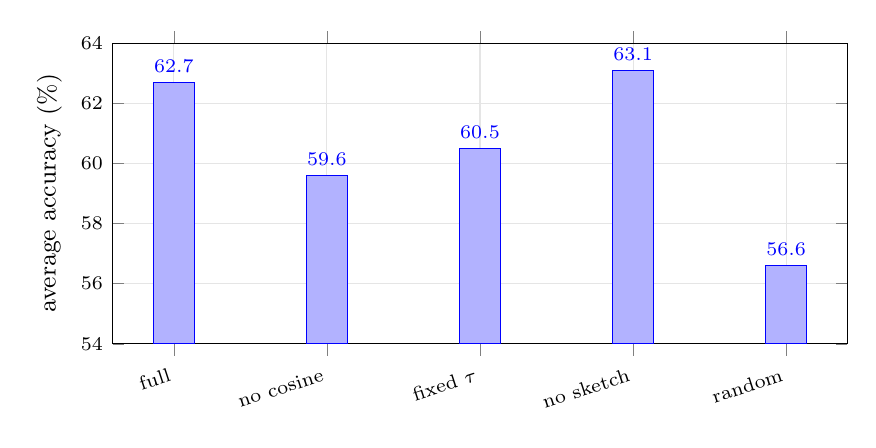
\begin{tikzpicture}
    \begin{axis}[
        width=0.9\linewidth, height=5.4cm,
        ybar, bar width=15pt,
        ylabel={average accuracy (\%)},
        symbolic x coords={full, no cosine, fixed $\tau$, no sketch, random},
        xtick=data,
        xticklabel style={font=\scriptsize,rotate=18,anchor=north east},
        ymin=54, ymax=64,
        nodes near coords, nodes near coords style={font=\scriptsize},
        grid=major, grid style={gray!20},
        tick label style={font=\scriptsize},
        label style={font=\small},
      ]
      \addplot coordinates {
        (full,62.7) (no cosine,59.6) (fixed $\tau$,60.5)
        (no sketch,63.1) (random,56.6)
      };
    \end{axis}
  \end{tikzpicture}
  \caption{Ablation at 7B, averaged over the four benchmarks. Scoring on full
  gradients is marginally better than the sketch and far more expensive.}
  \label{fig:ablation}
\end{figure}

\subsection{Anchor starvation}

Corollary~\ref{cor:anchor} predicts that anchored selection degrades below
roughly 120 anchor examples, and it does. Sweeping $m$ over
$\{32, 64, 128, 256, 512, 1024\}$ on \textsc{FinNER} at 1.4B gives 60.8, 61.1,
64.9, 66.8, 67.2, and 67.3 percent accuracy against a random-selection baseline
of 62.4. At $m = 64$ the method is 1.3 points below random. The failure is not
graceful, because a noisy anchor direction does not select randomly, it selects
consistently in a wrong direction and the curriculum then concentrates on that
direction for the whole early phase.

This is the practical limit of the method and we state it plainly. If a
deployment can supply only a few dozen target examples, the anchor should be
used for evaluation and the selection should be left uniform. A cheap guard is
available: bootstrap the anchor set, compute the alignment ranking on each
resample, and fall back to uniform sampling when the mean Spearman correlation
between resampled rankings falls below 0.4. That test flags $m = 64$ on all
four benchmarks and passes $m = 256$ on all four.

\subsection{Cost}

The scoring pass adds one forward and one backward per candidate per refresh.
At $P = 200$ steps and our budget this is 3.1 percent of total fine-tuning
FLOPs at 7B and 4.4 percent at 1.4B, where the projection is a larger fraction
of a smaller model's cost. Wall-clock overhead is slightly lower than the FLOP
count suggests because scoring is embarrassingly parallel and does not
synchronise across devices.
